%%%% CAPÍTULO 2 - REVISÃO DA LITERATURA (OU REVISÃO BIBLIOGRÁFICA, ESTADO DA ARTE, ESTADO DO CONHECIMENTO)
%%
%% O autor deve registrar seu conhecimento sobre a literatura básica do assunto, discutindo e comentando a informação já publicada.
%% A revisão deve ser apresentada, preferencialmente, em ordem cronológica e por blocos de assunto, procurando mostrar a evolução do tema.
%% Título e rótulo de capítulo (rótulos não devem conter caracteres especiais, acentuados ou cedilha)
\chapter{Fundamentação te\'orica}\label{cap:referencialTeorico}

Neste capítulo são apresentados alguns dos conceitos importantes para o entendimento
do trabalho. Sendo abordados assuntos como visão computacional, aprendizado de máquinas,
biometria e reconhecimento facial.

\section{SBC}\label{sec:formatacaoTexto}

O computador de placa única é um computador onde todos os componentes
necessários para sua operação estão localizados em uma única placa de circuito impresso. Esses
computadores são geralmente utilizados em sistemas de alarme, sistemas de medição, entre
outros.

Quando se trata de computadores de placa única, uma opção com ótimo custo beneficio 
é o ESP32. Não é o modelo mais potente, nem o mais compacto, ainda assim, possui muitos 
utilizadores devido sua simplicidade, poder de processamento e baixo consumo de corrente.

\begin{figure}[h!]
    \centering
    \caption{ESP32-DevKitC.}
    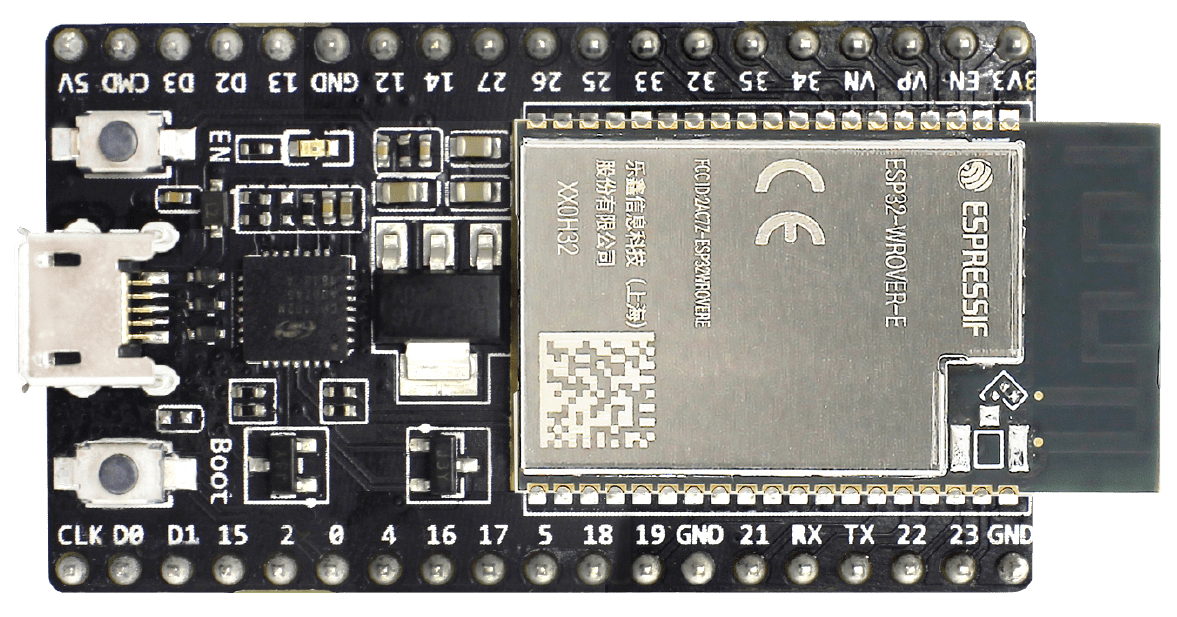
\includegraphics[scale=0.13]{figuras/esp323.png} 
    \legend{Fonte: Adaptado de \citeonline{espressifimg}.}
    \label{espzin}
    \centering
\end{figure}

A versão para este projeto será o ESP32-CAM, onde além de possuir um chip ESP32 
integrado, há também a câmera, entrada para cartão SD e LED de alto brilho.

\subsection{Arduino IDE}\label{sec:espacamento}

Uma forma para programar o ESP32 é utilizando o Arduino IDE.
Um software de código aberto, junto com um utilitário baseado em Python, também de código
aberto, chamado Esptool, que se comunica com o bootloader em chips Espressif ESP8266 e
ESP32.

\section{OPENCV}\label{sec:formatacaoTexto}

OpenCV é uma biblioteca de programação de código aberto originalmente da Intel com 
o objetivo de tornar a visão computacional mais acessível a desenvolvedores e amadores. 
Atualmente possui mais de 500 funções, pode estar em diferentes linguagens de programação e é 
utilizado para tipos de análise em imagens e vídeos, como detecção, rastreamento e 
reconhecimento facial, foto e edição de vídeo, detecção e análise de textos. (CEDRO, 2018).

\section{MÉTODO DE RECONHECIMENTO OPENCV}\label{sec:formatacaoTexto}

A primeira etapa do desenvolvimento é responsável por determinar qual modelo deve 
ser usado para detecção. Em seguida, uma instância da webcam é criada e a imagem da 
webcam é capturada no loop de repetição. (SCHMIDT, NOGUEIRA, 2015).

A detecção realmente ocorre usando a função detectMultiScale. Porém este método 
espera como parâmetro a imagem onde deve ser buscada as informações geométricas 
necessárias para uma boa detecção.

Deve-se tomar cuidado com a iluminação do local, para que não ocorra problemas na 
detecção. Pois mesmo com algoritmos e métodos sofisticados, ainda assim, perde-se algumas 
referências de posicionamento, ocasionando resultados com falsos positivos, ou falsos 
negativos.

\section{BIOMETRIA FACIAL PARA CONTROLE E ACESSO}\label{sec:formatacaoTexto}

A biometria facial é o recurso biométrico mais utilizado por humanos para identificação 
pessoal. A gama de aplicativos que usam esse recurso varia de aplicativos de reconhecimento 
facial estático em um ambiente controlado a imagens de fundo complexas de identidade em 
tempo.

As abordagens mais populares usadas no problema de reconhecimento facial são 
baseadas na localização e análise de atributos faciais como olhos, nariz e boca, ou em análise 
global destes, representada como uma combinação de uma série de faces canônicas.

Os sistemas de identificação baseados em biometria são essencialmente sistemas de 
reconhecimento que, dadas informações biométricas, são capazes de distinguir padrões e 
classificá-los em diferentes classes ou categorias.  (MORAES, 2010).

Ainda de acordo com o autor, algumas das principais características anatômicas, 
fisiológicas e comportamentais utilizadas em sistemas biométricos incluem impressão digital, 
impressão da mão, aparência facial, temperatura da face, retina, voz, assinatura, marcha e dental, 
entre outras.

Atualmente, nenhuma característica biométrica tem todas as propriedades de grau mais 
alto. Ou seja, não há "melhor característica" para um indivíduo. A escolha depende da aplicação 
em que será usada.

\section{TIPOS DE BIOMETRIA}\label{sec:formatacaoTexto}

De acordo com Moraes (2010), os principais tipos de biometria são:

Orelhas: Usa a anatomia da orelha para identificar indivíduos, abordagens incomuns. 
Os pontos fortes são aceitabilidade e permanência; fraquezas, singularidade e desempenho.

Termograma da face e das mãos: O padrão de calor emitido pelo corpo humano é uma 
característica de cada pessoa e pode ser captado por infravermelho. Sistemas baseados 
em imagens termográficas não requerem contato ou cooperação individual. No entanto, a 
captura de imagem continua sendo um desafio em ambientes não controlados, pois é afetada 
por fontes de calor que possivelmente podem estar próximas ao indivíduo. Seus pontos fortes 
são a universalidade, a impostura e a singularidade.

Impressão digital: recurso mais comumente usado em credenciais automatizadas em grande escala. 
Sua popularidade se deve em parte a dispositivos de coleta de baixo custo e desempenho de 
processo razoável. Embora a impressão digital não se modifique naturalmente ao longo dos anos, 
ela é sensível aos fatores ambientais aos quais os indivíduos estão submetidos, o que pode 
levar à sua alteração e deterioração. Trabalhadores manuais, por exemplo, podem ver suas 
impressões digitais constantemente alteradas devido a cortes profundos ou outros cortes em 
seus dedos.

Íris: Formada durante o desenvolvimento fetal, estabiliza-se durante os dois primeiros anos de 
vida. Sua textura é extremamente complexa e fornece informações a serem utilizadas no reconhecimento 
facial. Apresenta alta unicidade, sendo distinta mesmo em gêmeos idênticos. Tem um baixo grau de 
impostura, pois é difícil até cirurgicamente alterar a textura da íris. Seu ponto fraco está em sua 
capacidade de recuperação, requer equipamentos caros e complexos, bem como cooperação individual.

Voz: Combinação de biometria fisiológica e comportamental. Ele não muda em curtos períodos de tempo, 
mas é afetado por fatores como um simples frio, estado emocional e ruído de fundo. Possui baixa 
exclusividade e não é recomendado para identificação em larga escala. O ponto forte é a capacidade 
de coleta e aceitabilidade, além do baixo custo dos coletores. Geralmente indicado para verificação 
de identidade em conversas.

\section{RECONHECIMENTO FACIAL}\label{sec:formatacaoTexto}

Desde a infância, o ser humano adquire e desenvolve sua capacidade de reconhecer traços faciais, 
que é uma particularidade da visão, é o fundamento das relações sociais, atua como um dos principais 
fatores da evolução da espécie humana. As principais características da face humana foram retratadas 
relatadas há cerca de 27.000 anos atrás e durante esse período foram retratadas por inúmeros 
artistas. (ROUHANI, 2019).

Existem estudos sobre automatização do reconhecimento desde os anos 60. Os projetos iniciais nessa 
área dependiam do administrador encontrar manualmente as características faciais nas imagens, só 
então o sistema calculava as distâncias entre elas e comparava suas dimensões normalizadas com 
as referenciadas.

O processo de reconhecimento facial pode ser descrito a partir de uma imagem ou vídeo estático, 
identificar ou múltiplos indivíduos utilizando um banco de dados de rostos previamente cadastrados.
 Assim, existem três abordagens conhecidas para reconhecimento:

\begin{itemize}
    \item Imagem a imagem: a amostra e a base de dados composta por imagens estáticas;

    \item Vídeo para vídeo: a amostra e o banco de dados que consiste em vídeos;

    \item Imagem para vídeo: o exemplo é um vídeo. O vídeo é comparado a um banco de dados de 
    dados de imagens estáticas. A biblioteca OpenCV possibilita, a partir da versão 2.4, o 
    uso da classe FaceRecognizer para reconhecimento facial. Os algoritmos atualmente disponíveis 
    na biblioteca são: Fisherfaces e Histogramas de Padrões Binários Locais.
\end{itemize}